\chapter{Development of the Cube}
\myTop{
In this chapter the development and the problematics with the patenting and legal issues regarding the cube are described. The purpose of this chapter is to give the reader a basic understanding of the \rubik{}.
}
\erno{} is the inventor behind the world famous \rubik{}. He was born in Budapest, Hungary in 1944.  In college he studied sculpture. After his graduation he started studying architecture.  Once he graduated with a degree in architecture he stayed at the college to teach interior design.

Rubik got the idea for the cube when he wanted to make a 3D design with blocks that could move individually but many at the same time. Rubik initially tried  to make a cube that was held together with rubber bands but failed. Then he got the idea that the cubes had to hold each other in place, which resulted in a 2x2x2 cube that could \twist{} each \face{} individually. Rubik got the inspiration for the cube from the Magic Puzzle (see chapter \ref{chap:recreationalMathematics}). At first the cube was named the Magic Cube. The company Ideal Toy bought exclusive rights for the Magic Cube, but changed the name of the cube to \rubik{} within a year in order to get trademark protection.

Rubik described that some of the most important features behind the cube were that the parts of the cube stay together, which many other puzzle do not. He also pointed out that you can move several pieces at once. Also that it is three dimensional. 

In \myDate{}{1}{1975} Rubik applied for a patent for his invention in Hungary. Two years later in 1977 he got the patent on the \rubik{}.

At that time there were also two others applying for patent for products similar to the \rubik{}.  One of them was an American named Doctor Larry D. Nichols, and his cube was a 2x2x2 cube which was held together with magnets. The other one who applied for patent was a Japanese man named Terutoshi Ishige. He applied for patent a year after Rubik. Terutoshi Ishige's cube was almost identically to the \rubik{}. 

In the 80s he became professor with full tenure, and in 1990 he became the president of the Hungarian Engineering Academy. He created the International Rubik Foundation to support especially talented young engineers and industrial designers.
 
\section{Rubik's Cube(Magic Cube)}

 In the 70s Ern? Rubik was teaching in Interior Design at Academy of Applied Arts and Crafts and he was trying to find at tool to help his students to understand 3D objects as result he made the magic Cube in 1974 and obtained a Hungarian patent HU170062 for it in 1975.

In the end of 70s a Hungarian Businessman show the Magic Cube at the Nuremberg toy fair end made it popular in Europe. In 1979 Ideal Toy Company bought the rights to the Magic Cube and changed the name to Rubik's Cube and made trademark protection. 

Ideal Toy Company were bought by CBS Toy Company in 1982 at the trademark surpassed with it, but they sold the rights to Rubik's Cube to Seven Towns there is a Toy Company in Great Britain, they are still producing  The Rubik's Cube today.


 
\section{The Nichols Cube Puzzle}
Dr. Larry D. Nichols studied chemistry at DePauw University in Greencastle, Indiana, before moving to Massachusetts to attend Harvard Graduate School. 
He is a lifelong puzzle enthusiast and inventor who  began developing a twist cube puzzle with six colored faces in 1957. It was made of eight smaller cubes assembled to a 2x2x2 cube. The eight cubes were held together by magnets.

\begin{figure}[H]
\begin{center}
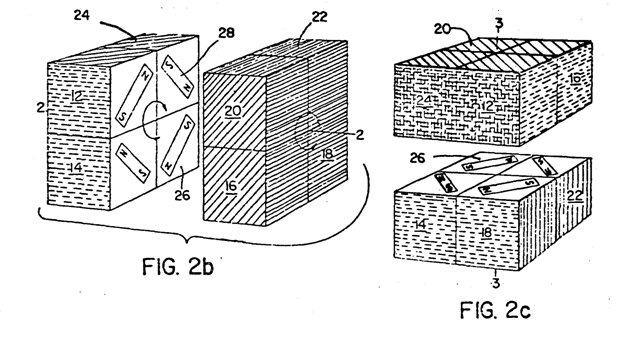
\includegraphics[scale=0.8]{input/pics/Nicholspatent2.png}
\caption{\myCaption{Figure of Nichols Patent.}}
\label{fig:Nicholspatent}
\end{center}
\end{figure}

On \myDate{11}{4}{1972} he was granted U.S. Patent 3,655,201 on behalf of Moleculon Research Corp. U.S. Patent 3,655,201 covered Nichols Cube and the possibility for making larger versions later. This was two years before \erno{} took out the patent for his \rubik{}. 

In 1982 Moleculon Research corp.  Sued Ideal Toy Company that had the U.S. Patent 4,378,116 for \rubik{} because they believed that Ideal Toy Company violated their patent, but the U.S. District Court ruled in Ideal Toy Company favor. In 1986 the Court of Appeals ruled that the Pocket \rubik{} 2x2x2 was guilty of infringement but not the 3x3x3 \rubik{}.
